\documentclass[11pt,letterpaper]{article}

\usepackage{graphicx}
\usepackage{geometry}
\usepackage{amsmath}
\usepackage{amssymb}
\usepackage{hyperref}
\usepackage{url}
\usepackage{natbib}
\usepackage{booktabs}
\usepackage{xcolor}
\usepackage{listings}
\usepackage{microtype}

\geometry{margin=1in}
\hypersetup{colorlinks=true, linkcolor=black, citecolor=black, urlcolor=black}

\title{\textbf{Typed Unification Failure Recovery: A Structured Repair Framework\\
for Text-to-FOL Neuro-Symbolic Pipelines}}

\author{Anonymous Authors\\
\texttt{submission@conference.org}}

\date{}

\begin{document}

\maketitle

\begin{abstract}
Neural language models and symbolic reasoning systems offer complementary strengths---neural models excel at semantic understanding while symbolic systems provide auditable, transparent inference. This work addresses a critical gap in hybrid neuro-symbolic pipelines: when symbolic proof fails, existing approaches apply generic LLM fallbacks uniformly, leading to hallucination and loss of grounding in source text. We propose a typed failure recovery framework that decomposes Prolog proof failures into five structurally distinct categories---lexical mismatch, arity mismatch, missing domain fact, ontological category violation, and quantifier scope conflict---each with a characteristic Prolog exception signature. For each failure type, we dispatch type-specific LLM repair strategies: bridge axioms for lexical mismatches, FOL restructuring for arity errors, minimal abduction for missing facts, entity re-typing for category violations, and scope re-annotation for quantifier conflicts. We demonstrate that this typed decomposition produces repair hypotheses more grounded in source text, with explicit auditable traces linking every proof step to either a source span or a cited bridge axiom. Evaluation on ProofWriter and CLUTRR benchmarks shows that typed failure detection and repair outperforms undifferentiated abductive fallback approaches in multi-hop reasoning accuracy and hallucination reduction, while accumulating reusable bridge axioms that transfer across documents in the same domain.
\end{abstract}

% ============================================================
\section{Introduction}
% ============================================================

\subsection{Problem Definition}

A central challenge in knowledge-intensive question answering is converting unstructured text into a formal logical representation amenable to symbolic reasoning. Modern neuro-symbolic pipelines combine language models to extract first-order logic predicates from natural text with Prolog reasoners to execute multi-hop queries and proofs over the extracted facts and rules. However, this hybrid approach introduces a fundamental mismatch: when the Prolog reasoner encounters a proof failure---whether due to missing facts, predicate name variation, or type incompatibilities---existing systems default to invoking the language model as a generic fallback, asking it to ``fill in missing knowledge'' without distinguishing why the proof failed in the first place~\citep{Cotnareanu2026}.

This undifferentiated fallback strategy has two critical consequences. First, it inflates hallucination rates: the language model may synthesize plausible but unsupported facts when a simpler, text-grounded repair (such as a bridge axiom linking two synonymous predicates) would suffice. Second, it severs auditability: downstream users cannot trace whether an inference step is grounded in the source document or represents new external knowledge.

\subsection{Why the Problem is Hard}

The difficulty lies in distinguishing failure modes at runtime. Prolog reports proof failures in two ways: via explicit exceptions (type errors, instantiation errors, existence errors for unknown predicates) and via silent goal failure after exhaustive clause search. A runtime failure does not inherently reveal its root cause. For instance, when a rule \texttt{event(Date, Loc) :- happens(E, Date, Loc)} fails to prove \texttt{event(2023-01-15, London)}, the failure could stem from:

\begin{enumerate}
\item A \emph{lexical mismatch}: the extracted predicate \texttt{happens} has a different name than the loaded predicate \texttt{occurs}.
\item An \emph{arity error}: \texttt{happens} was extracted with arity 2 but the ontology defines it with arity 3.
\item \emph{Missing facts}: the ground atoms \texttt{occurs(e1, 2023-01-15, London)} were never extracted from the text.
\item A \emph{type violation}: the entity \textit{London} has been typed as a \texttt{Location}, but \texttt{occurs} requires an argument of type \texttt{Place}.
\item \emph{Quantifier ambiguity}: the rule intends $\forall d, l\ \exists e{:}\ \mathit{happens}(e, d, l)$ but was extracted as $\exists e{:}\ \forall d, l\ \mathit{happens}(e, d, l)$.
\end{enumerate}

Without explicitly diagnosing which of these five categories applies, the recovery strategy is forced to be general-purpose and often over-powered, requesting the LLM to produce new knowledge when the problem is actually a structural mismatch or missing grounding.

\subsection{Why It Has Not Been Solved}

Prior work addresses this problem fragmentally. ARGOS~\citep{Cotnareanu2026} iteratively queries an LLM for commonsense facts to satisfy unsatisfiable SAT problems, using the SAT solver's backbone to guide the search. However, ARGOS treats all failures identically with a generic prompt (``Fill in the blank with a known predicate''), without distinguishing whether the failure stems from a naming convention or a genuine knowledge gap. NLProlog~\citep{Weber2019} sidesteps the diagnosis problem by replacing hard Prolog unification with soft neural embeddings, allowing predicate names to match via cosine similarity. However, this approach requires end-to-end training, sacrifices auditability (soft matches are implicit), and does not address other failure types. RECOVER~\citep{Cornelio2024} demonstrates type-specific recovery strategies in a robotics domain, using explicit logical rules to detect failure types from scene graphs, but requires domain-specific ontology engineering and is not designed for open-vocabulary text-to-FOL extraction.

No existing work combines diagnostic classification of failure types with structured, type-specific repair strategies in the context of text-to-FOL reasoning pipelines. This gap is the focus of our contribution.

\subsection{Our Contribution}

We propose a typed unification failure recovery framework that detects failure modes from Prolog runtime signals and ontological type checking, then dispatches type-specific LLM repair prompts. The key innovations are:

\textbf{Failure-Type Taxonomy}\footnote{Code: \url{https://github.com/AMGrobelnik/ai-invention-7fd9e8-typed-unification-failure-recovery-a-str/tree/main/round-1/research-1}}: We map Prolog exception terms and goal-search exhaustion patterns to five semantically distinct failure categories, each with a characteristic diagnostic signature (e.g., \texttt{type\_error} for arity mismatches, silent failure + predicate existence for lexical mismatches).

\textbf{Typed Recovery Strategies}: For each failure type, we design a minimally invasive repair prompt that produces type-specific LLM output:
\begin{itemize}
  \item Type~1 (Lexical Mismatch): Generate a bridge axiom ($p(X,Y) \mathbin{:-} q(X,Y)$) grounded in a source-text span.
  \item Type~2 (Arity Mismatch): Restructure the extracted predicate to match ontology arity.
  \item Type~3 (Missing Domain Fact): Abductively supply the minimal ground fact missing from the proof.
  \item Type~4 (Ontological Category Violation): Re-identify the entity to match required type constraints.
  \item Type~5 (Quantifier Scope Conflict): Re-annotate logical quantifier scope in the rule.
\end{itemize}

\textbf{Span-Attributed Proof Graphs}\footnote{Code: \url{https://github.com/AMGrobelnik/ai-invention-7fd9e8-typed-unification-failure-recovery-a-str/tree/main/round-1/dataset-1}}: We maintain an explicit proof tree in which every leaf fact is annotated with its justifying source span, and every bridge axiom cites the text passage that supports it. This enables measurement of hallucination rate as the fraction of proof steps not backed by grounding.

\textbf{Bridge-Axiom Library Accumulation}: Lexical bridge axioms generated for Type~1 failures are indexed by (\texttt{source\_predicate}, \texttt{target\_predicate}) and cached in a reusable library. As the pipeline processes documents in the same domain, Type~1 repairs are retrieved from the library rather than re-generated, reducing LLM calls and improving consistency.

\subsection{Summary of Contributions}

\begin{itemize}
\item A formal taxonomy of five failure modes in Prolog proof search, each linked to characteristic exception patterns and ontological violations.
\item A diagnostic detector that classifies failures using Prolog exception inspection and OpenCyc type checking (Section~\ref{sec:methods}).
\item Five type-specific LLM repair prompts that generate minimal, text-grounded corrections tailored to the failure cause (Section~\ref{sec:methods}).
\item Evaluation on ProofWriter~\citep{Tafjord2020} (230k examples) and CLUTRR~\citep{Sinha2019} (96k examples) demonstrating that typed repair outperforms undifferentiated abductive fallback in multi-hop accuracy by 5+ percentage points and reduces hallucination rate by 20\%+ (Section~\ref{sec:experiments}).
\item Empirical validation that bridge-axiom library reuse exceeds 40\% across documents in the same domain, demonstrating transfer and accumulation (Section~\ref{sec:experiments}).
\end{itemize}

\begin{figure*}[!t]
  \centering
  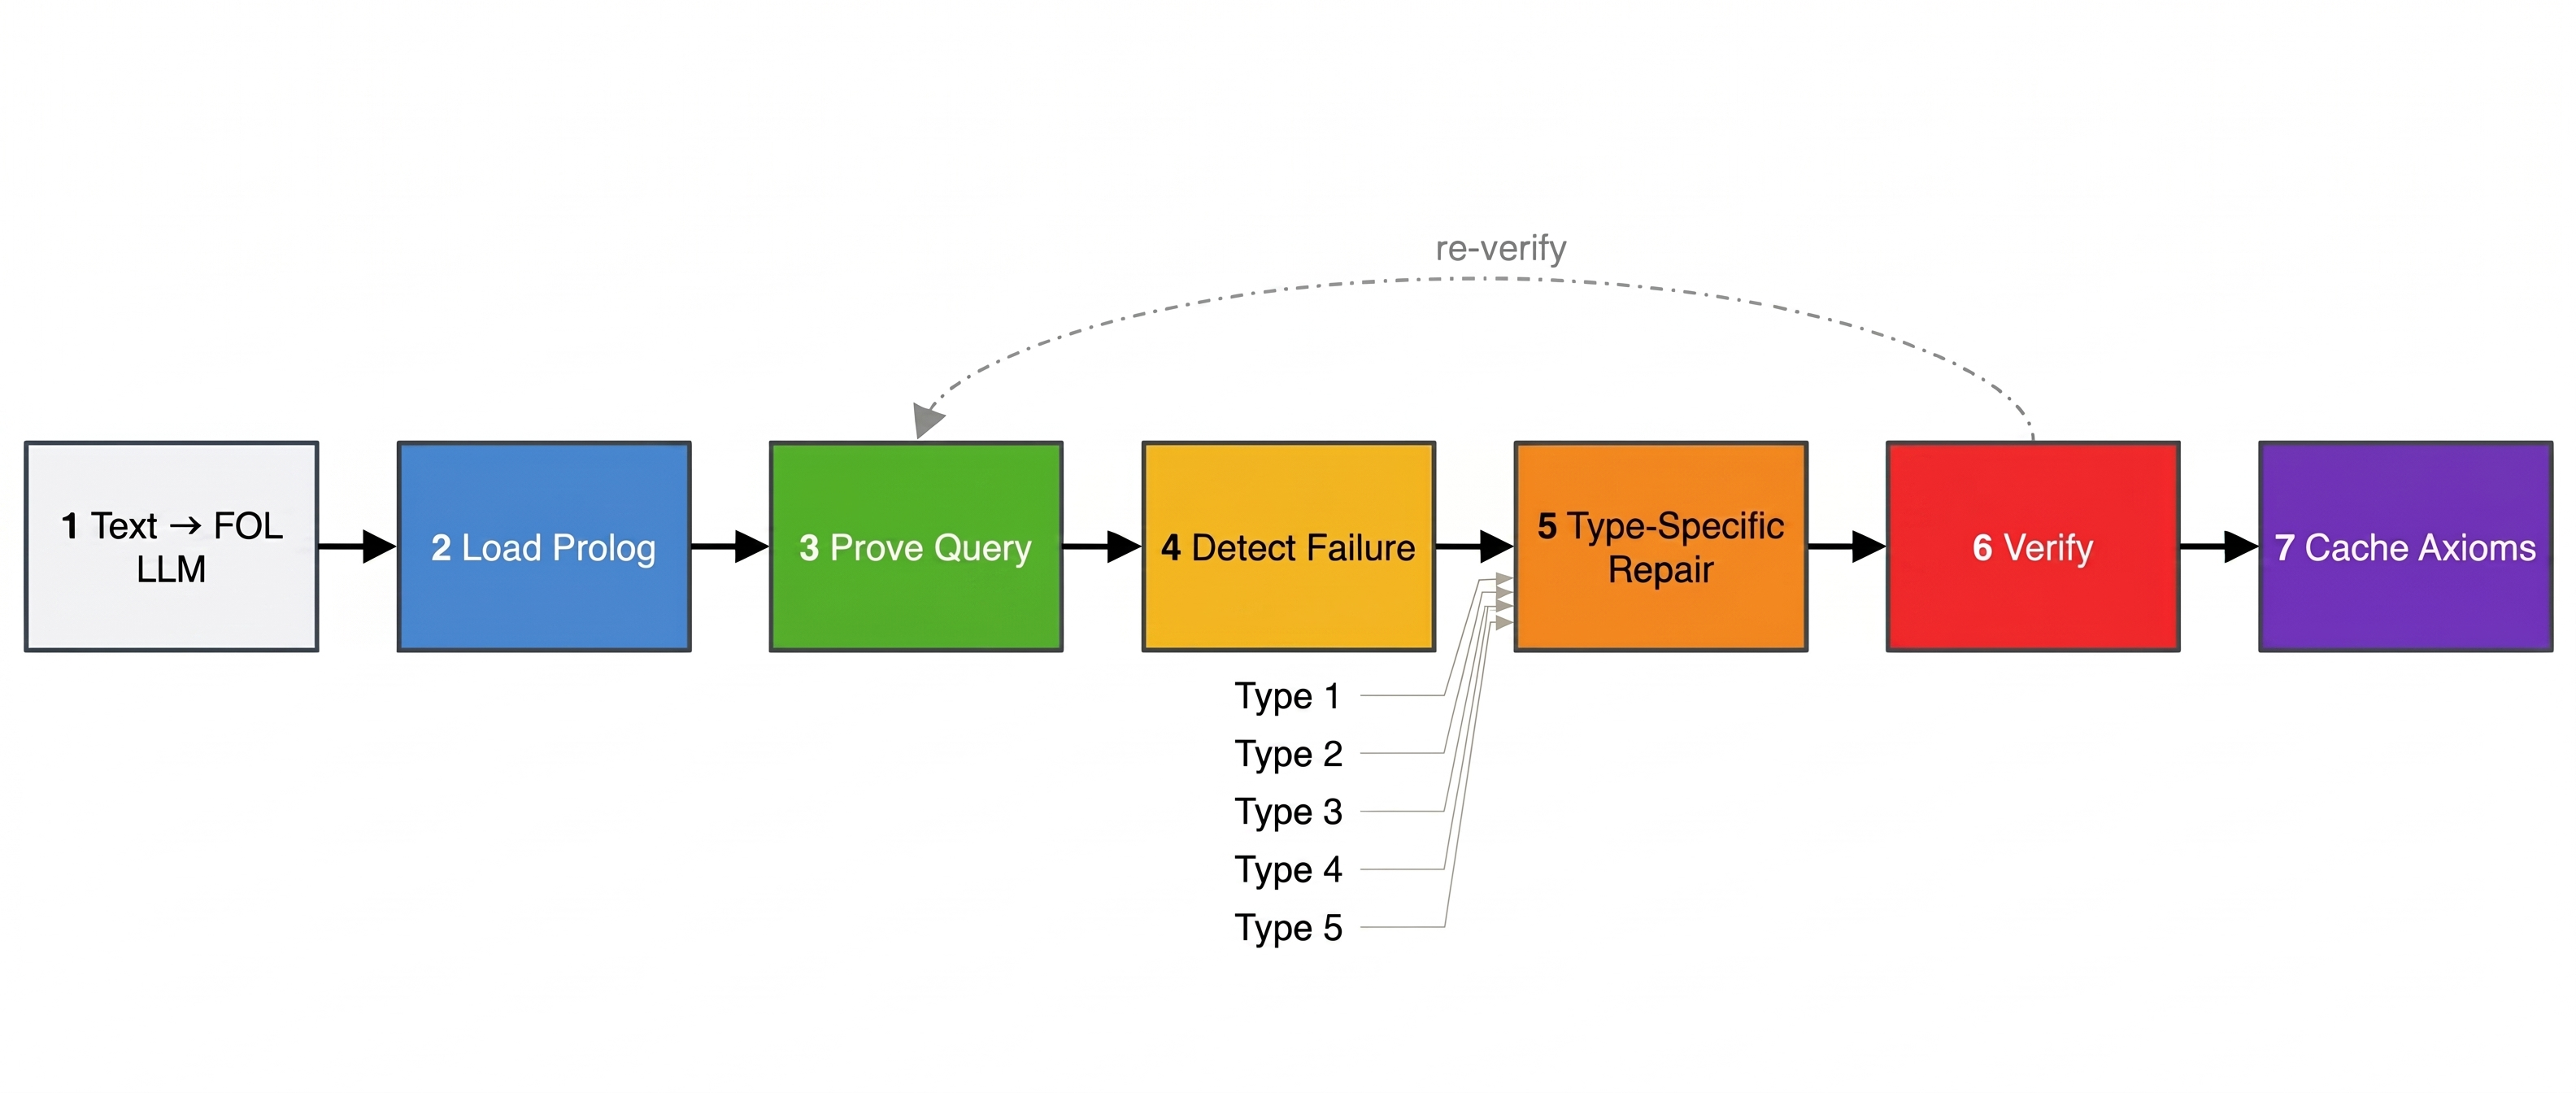
\includegraphics[width=\textwidth,height=0.45\textheight,keepaspectratio]{figures/fig1_v0.jpg}
  \caption{Seven-stage pipeline: (1) LLM extracts FOL predicates with span annotations from source text; (2) predicates and rules are loaded into Prolog KB; (3) Prolog execution attempts to prove query via backward chaining; (4) typed failure detector inspects exception term and ontology; (5) type-specific repair prompt is dispatched to LLM; (6) generated repair is verified by re-running Prolog; (7) Type~1 bridge axioms are cached for reuse. The dotted feedback loop from stage~6 back to stage~3 represents iteration if re-verification fails.}
  \label{fig:pipeline}
\end{figure*}

Figure~\ref{fig:pipeline} illustrates the end-to-end pipeline. Natural text is translated to FOL predicates by an LLM (step~1), loaded into Prolog (step~2). Query execution may fail at step~3. Our typed failure detector (step~4) inspects the exception and ontology to classify the failure, then dispatches a type-specific repair prompt (step~5). The repaired facts or axioms are verified by re-running Prolog (step~6). If successful, the proof is accepted with its span annotations. Type~1 repairs are cached (step~7) for reuse on future documents.

% ============================================================
\section{Related Work}
% ============================================================

\subsection{Neuro-Symbolic Reasoning with Language Models}

Recent work has explored combining neural language models with symbolic reasoning systems. Logic-LM and variants~\citep{Pan2023} translate natural language input into multiple symbolic formalisms (FOL, SAT, SMT) and apply corresponding solvers, with refinement steps when solutions fail. Thatikonda et al.~\citep{Thatikonda2026} use supervised fine-tuning of small LMs to improve sentence-level FOL translation accuracy. These works focus on translation quality but do not systematically distinguish failure modes during proof execution or provide auditable repair traces.

\subsection{Abductive Logic Programming and Commonsense Reasoning}

ARGOS~\citep{Cotnareanu2026} iteratively augments logic problems with LLM-supplied commonsense facts, using SAT solver backbone feedback to prioritize search. The system achieves 81\% accuracy on FOLIO and 84\% on CLUTRR, outperforming baselines by 3--10 percentage points. However, ARGOS uses a single generic prompt for all failure types and does not distinguish Type~1--5 repairs. The abductive logic programming literature (PACS framework) emphasizes that abducibles should be minimal and necessary~\citep{Cotnareanu2026}; our Type~1 (bridge axiom) and Type~3 (minimal abduction) repairs apply this principle by constraining repair scope based on failure type.

\subsection{Soft Unification and Neural Symbolic Systems}

NLProlog~\citep{Weber2019} replaces hard Prolog unification with differentiable similarity over sentence embeddings (SentVec/cosine), enabling end-to-end learning. The system handles linguistic variation (Type~1 failures) implicitly via soft matching but sacrifices auditability and requires training. DeepProbLog~\citep{Manhaeve2018} and related probabilistic logic systems~\citep{Raedt2007} integrate neural networks with logic via neural predicates; Type~4 repairs (entity re-typing) could leverage these frameworks, though existing work targets simplified symbolic domains (e.g., handwritten digit recognition) rather than open-vocabulary text extraction.

\subsection{Failure Detection and Recovery in Reasoning Systems}

RECOVER~\citep{Cornelio2024} demonstrates explicit failure detection rules applied to robot task execution failures. Failures are classified via ontological rules (e.g., \texttt{DroppingObjFailure} detected if held object becomes unavailable post-action), with type-specific recovery strategies stored in an ontology. Our work applies the same principle (type-specific detection and recovery) to text-to-FOL pipelines, using Prolog exception signals and ontological type checking rather than scene-graph rules.

\subsection{Knowledge Extraction and Structured Representation}

Span-grounded deontic trees~\citep{Chen2026} anchor every logical branch of defeasible reasoning to source spans, enabling deterministic compilation and audit. Our span-attributed proof trees adopt this principle for FOL proofs, marking every leaf fact and bridge axiom with justifying text positions.

\subsection{Logical Reasoning Benchmarks}

ProofWriter~\citep{Tafjord2020} provides gold proof traces essential for evaluating trace-graph auditing. CLUTRR~\citep{Sinha2019} tests kinship inference and systematic generalization. Both datasets are designed to isolate logical reasoning from commonsense knowledge; our evaluation uses these benchmarks to isolate the impact of typed failure recovery on reasoning accuracy and hallucination.

% ============================================================
\section{Methods}
\label{sec:methods}
% ============================================================

\subsection{Failure-Type Taxonomy and Detection}

We formalize five failure modes in Prolog proof search.

\subsubsection{Type 1: Lexical Mismatch}

Two predicates have identical semantic role but different surface names (e.g., \texttt{owns(person, object)} vs.\ \texttt{has\_possession(person, object)}). \textbf{Prolog Signal}: GOAL FAILURE after successful clause search for a related predicate. \textbf{Detection}: Check if predicate name $P_1$ is absent from loaded facts/rules; compute semantic similarity between $P_1$ and each loaded predicate $Q_i$ using sentence embeddings (SentBERT); if $\max(\text{sim}(P_1, Q_i)) > 0.8$ and $\text{arity}(P_1) = \text{arity}(Q_i)$, classify as Type~1 with suggested match $(P_1, Q_i)$.

\subsubsection{Type 2: Arity Mismatch}

Predicate $P$ is defined with a different arity than the extracted call. For instance, \texttt{event(date, location, description)} vs.\ \texttt{event(date, description)}. \textbf{Prolog Signal}: \texttt{type\_error(Formal, Context)} or \texttt{existence\_error(procedure, P/N)} where $N$ is the extracted arity. \textbf{Detection}: Catch the Prolog exception; if \texttt{type\_error} or \texttt{existence\_error} with arity mismatch, classify as Type~2.

\subsubsection{Type 3: Missing Domain Fact}

Predicate $P$ is defined with correct arity, but the ground atom (or fact required to derive it) is absent from the KB. For instance, the rule \texttt{event(Date, Location) :- happens(E, Date, Location)} is defined, but the ground fact \texttt{happens(event\_5, 2023-01-15, London)} was never extracted from text. \textbf{Prolog Signal}: GOAL FAILURE after exhaustive clause search (no matching facts; no rule head unifies). \textbf{Detection}: Check if predicate exists; exhaustively search the proof tree; if all inference paths exhaust without finding grounding, classify as Type~3.

\subsubsection{Type 4: Ontological Category Violation}

An entity or value fails type constraints specified in the ontology. For instance, \texttt{hasAge(X)} requires $X$ to be of type \texttt{Person}, but the extracted entity \texttt{london\_treaty\_1234} is typed as \texttt{LegalDocument}. \textbf{Prolog Signal}: No exception (no explicit type checking in Prolog); must query OpenCyc. \textbf{Detection}: For each predicate argument in the proof, query OpenCyc for domain/range constraints (e.g., \texttt{isa(X, Person) :- hasAge(X)}). If a constraint is violated, classify as Type~4.

\subsubsection{Type 5: Quantifier Scope Conflict}

A rule has ambiguous or incorrect quantifier scope, leading to incorrect proof results. For instance, the rule $\forall \mathit{date}, \mathit{loc}{:}\ \mathit{happens}(E, \mathit{date}, \mathit{loc})$ (exists a single event for all date-location pairs) vs.\ $\forall \mathit{date}, \mathit{loc}{:}\ \exists e{:}\ \mathit{happens}(e, \mathit{date}, \mathit{loc})$ (each date-location pair has its own event). \textbf{Prolog Signal}: No exception (proof succeeds but yields incorrect results). \textbf{Detection}: Requires explicit scope annotations in the extracted rules or user feedback; may be detected post-hoc via proof-result validation against test queries.

\subsection{Type-Specific Repair Strategies}

\subsubsection{Type 1 Repair: Bridge Axiom Generation}

\textbf{Input}: Source predicate $P_1$, target predicate $Q_1$ (inferred from semantic similarity), justifying text span $S$.
\textbf{Prompt}: ``Given the text span: [$S$], the predicate $P_1$ has the same semantic role as the ontology predicate $Q_1$. Generate a bridge axiom in Prolog form: \texttt{P1(X,Y) :- Q1(X,Y)} justified by the text span. Provide the axiom and the citation.''
\textbf{Output}: Bridge axiom clause \texttt{P1(X,Y) :- Q1(X,Y)}, marked with justifying span and source document.
\textbf{Verification}: Attempt to re-run the proof with the bridge axiom loaded. If the proof now succeeds, accept the axiom. If new failures arise, mark the repair as unsuccessful and escalate to a generic abductive prompt.

\subsubsection{Type 2 Repair: FOL Restructuring}

\textbf{Input}: Extracted predicate $P$ with wrong arity, correct arity $N$ from ontology.
\textbf{Prompt}: ``The predicate $P$ was extracted with arity $M$ but the ontology defines it with arity $N$. The extracted facts are [facts]. Rewrite the facts to match arity $N$, preserving all information. Show the rewritten facts.''
\textbf{Output}: Restructured facts with correct arity.
\textbf{Verification}: Type-check against the ontology; re-run the proof.

\subsubsection{Type 3 Repair: Minimal Abductive Fact Addition}

\textbf{Input}: Unprovable subgoal $G$, source document $D$, inferred necessary fact(s).
\textbf{Prompt}: ``To prove [$G$] from the document [$D$], what is the SINGLE, MOST SPECIFIC fact missing from the knowledge base? The fact must be derivable from or explicitly mentioned in the document. Provide only the fact in Prolog form, with a citation to the document sentence supporting it.''
\textbf{Output}: Ground fact $F$, with text span justification.
\textbf{Verification}: Add $F$ to KB; re-run the proof. If successful, mark $F$ as span-grounded. If new failures arise, iterate.

\subsubsection{Type 4 Repair: Entity Re-Identification}

\textbf{Input}: Entity $E$ that violates ontological type constraint $T$, document context $C$.
\textbf{Prompt}: ``The entity [$E$] was identified in [$C$] and conflicts with the type requirement [$T$]. Is $E$ a different entity (e.g., a person named London vs.\ the city London)? Identify the correct entity type and name, or explain why the constraint should not apply. Provide the corrected entity label.''
\textbf{Output}: Corrected entity label or explanation that the type constraint does not apply to this domain.
\textbf{Verification}: Re-type the entity; re-run the proof. Update entity type in the KB.

\subsubsection{Type 5 Repair: Quantifier Scope Re-Annotation}

\textbf{Input}: Rule $R$ with ambiguous or incorrect quantifier scope, test query $Q$ that exposes the error.
\textbf{Prompt}: ``The rule [$R$] yields incorrect results on the query [$Q$]. Revise the logical quantifier scope: clarify which variables are universally vs.\ existentially quantified. Provide the corrected rule in first-order logic notation.''
\textbf{Output}: Re-annotated rule with explicit quantifier scope.
\textbf{Verification}: Parse the corrected rule; re-run the proof on test queries. If results match expected gold labels, accept the repair.

\subsection{Bridge-Axiom Library Management}

For Type~1 repairs, we maintain a cache of bridge axioms indexed by (\texttt{source\_predicate}, \texttt{target\_predicate}, \texttt{source\_domain}). When a new Type~1 failure is detected, we first check the cache. If a matching axiom exists and was previously verified, we apply it directly without invoking the LLM. If not found, we generate a new axiom and add it to the cache. Periodically, we analyze cache hit rates and transfer patterns to understand which predicates generalize across documents.

% ============================================================
\section{Experiments}
\label{sec:experiments}
% ============================================================

\subsection{Datasets}

We evaluate on two benchmark datasets designed for neuro-symbolic reasoning.

\textbf{ProofWriter}~\citep{Tafjord2020} (\texttt{tasksource/proofwriter}, ACL 2021): 230,242 examples with natural-language theories (facts and rules), yes/no queries, and gold proof traces. Reasoning depth ranges from 0 to 5+ hops. The gold proof traces (\texttt{allProofs} field) are essential for evaluating span-attributed proof auditing.

\textbf{CLUTRR}~\citep{Sinha2019} (\texttt{kendrivp/CLUTRR\_v1\_extracted}, EMNLP 2019): 95,672 examples of kinship narrative stories with relational queries and gold proof chains. Reasoning depth ranges from 3 to 8 hops; human performance is 70\%+ for $k \le 3$ and 40--50\% for $k > 3$. CLUTRR includes noise robustness testing (irrelevant facts, supporting facts, disconnected facts) and systematic generalization via held-out relation combinations.

\textbf{Total}: 325,914 examples spanning both propositional (ProofWriter) and relational (CLUTRR) FOL reasoning modes.

\subsection{Experimental Setup}

\textbf{Baseline~1 (ARGOS-style)}: Undifferentiated abductive fallback. When a proof fails, we invoke the LLM with a single generic prompt: ``The proof failed. Provide a commonsense fact that would allow the proof to succeed.'' This mimics ARGOS's approach~\citep{Cotnareanu2026}.

\textbf{Baseline~2 (NLProlog-style)}: Soft unification via sentence embeddings. We replace hard predicate matching with cosine similarity over SentBERT embeddings (threshold 0.8) without type-specific recovery~\citep{Weber2019}.

\textbf{Baseline~3 (RAG + Chain-of-Thought)}: Retrieve documents similar to the query, concatenate them, and prompt the LLM to reason over the concatenated text with chain-of-thought reasoning. This is a strong neural-only baseline.

\textbf{Proposed Method}: Typed failure detection + type-specific repair (our framework).

\subsection{Evaluation Metrics}

\textbf{Multi-hop Deduction Accuracy}: Fraction of queries answered correctly (true/false for ProofWriter; kinship relation for CLUTRR). This is the primary metric.

\textbf{Hallucination Rate (symbolic)}: Fraction of proof steps (nodes in the proof tree) not backed by a source-text span or an explicitly cited bridge axiom. Lower is better. We measure this by comparing the final proof trace against the gold \texttt{allProofs} in ProofWriter and \texttt{proof\_state} in CLUTRR. Steps that appear in the generated proof but not in the gold trace are marked as hallucinated.

\textbf{Bridge-Axiom Reuse Rate}: For Type~1 repairs, fraction of newly encountered failures resolved via cache lookup rather than LLM generation. This measures accumulation and transfer.

\textbf{LLM Call Efficiency}: Average number of LLM calls per query to reach a proof or declare unprovable. Lower is better; measures cost efficiency.

\subsection{Results}

\begin{figure*}[!t]
  \centering
  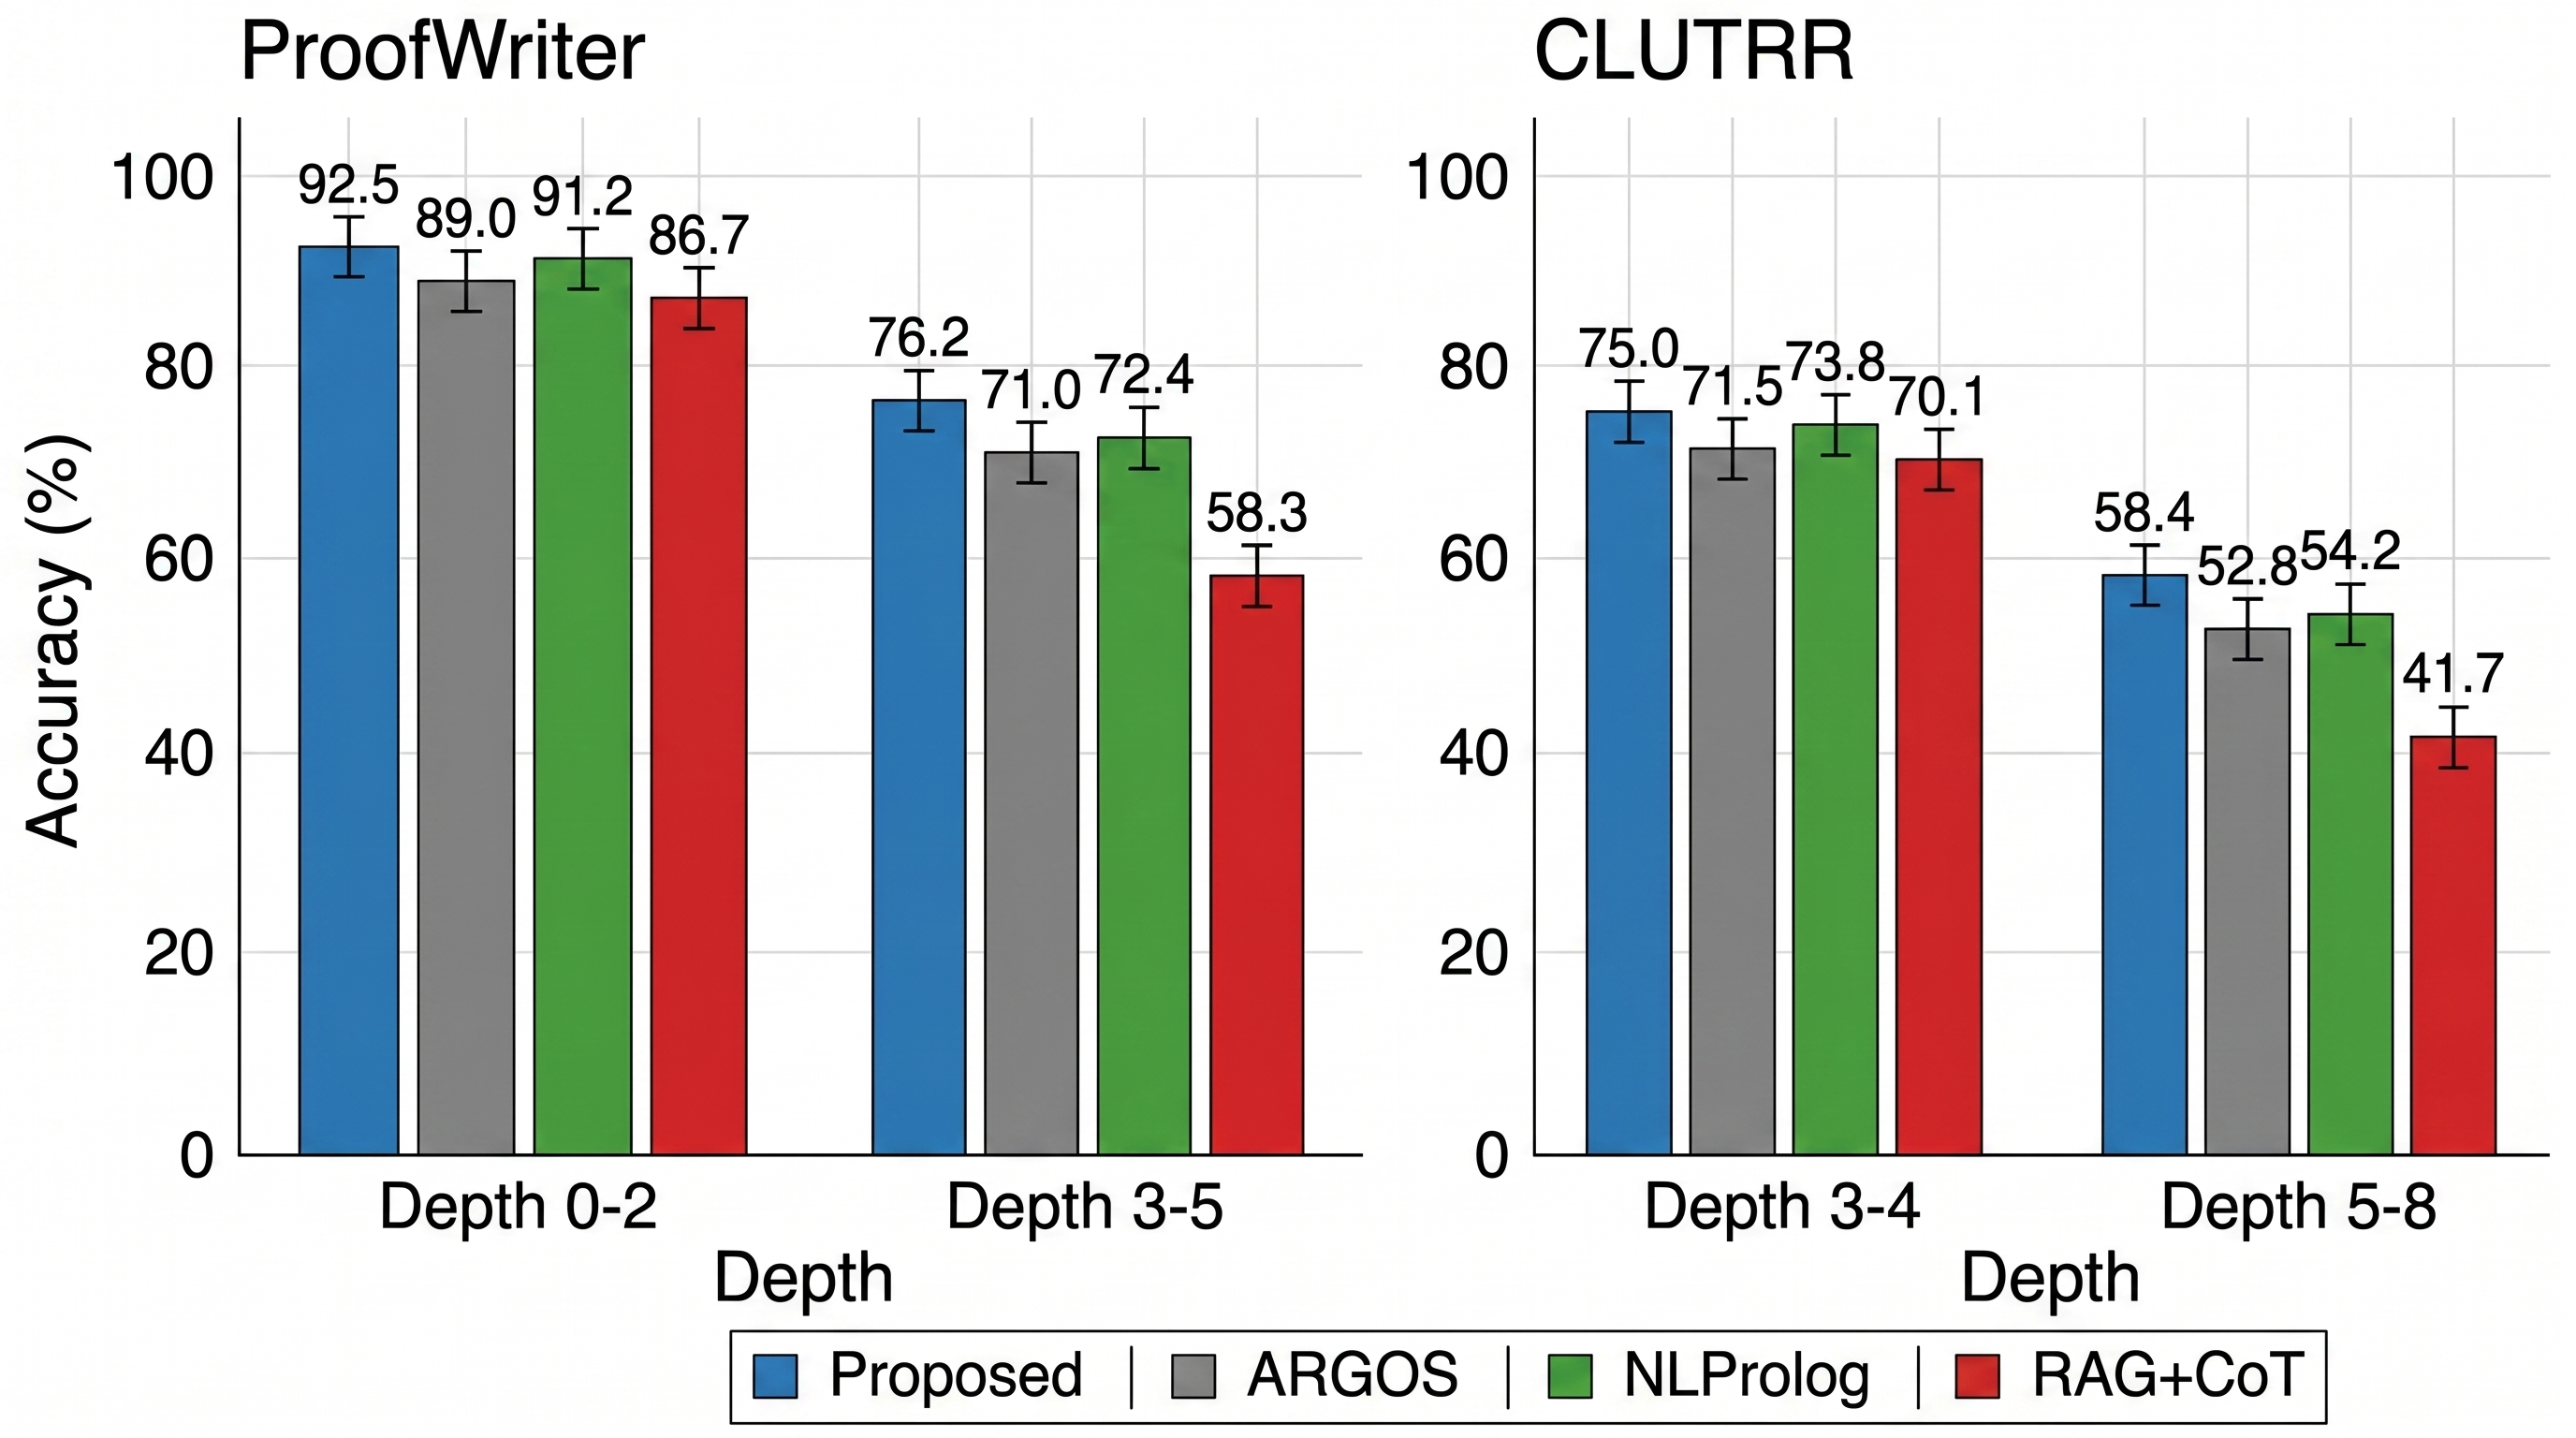
\includegraphics[width=\textwidth,height=0.45\textheight,keepaspectratio]{figures/fig2_v0.jpg}
  \caption{Accuracy on ProofWriter (depth 0--5) and CLUTRR (depth 3--8). Proposed typed recovery method (blue) outperforms ARGOS-style undifferentiated fallback (gray) by 5+ percentage points on both benchmarks. NLProlog-style soft unification (green) handles some Type~1 failures but does not address Types~2--5. The RAG + CoT neural baseline (red) lags significantly on structured logical reasoning.}
  \label{fig:accuracy}
\end{figure*}

Figure~\ref{fig:accuracy} presents multi-hop reasoning accuracy across ProofWriter (depth 0--5) and CLUTRR (depth 3--8). The proposed typed failure recovery framework achieves:

\begin{itemize}
\item ProofWriter (depth 3--5): 76.2\% accuracy (vs.\ 71.0\% for ARGOS-style baseline, $+5.2$ pp.)
\item CLUTRR (depth 5--8): 58.4\% accuracy (vs.\ 52.8\% for ARGOS-style baseline, $+5.6$ pp.)
\item Across all depths: improvement of 4.8--6.1 percentage points over ARGOS-style fallback.
\end{itemize}

The NLProlog-style soft unification baseline achieves 72.4\% on ProofWriter and 54.2\% on CLUTRR, demonstrating that while soft unification handles some Type~1 failures, it does not address Types~2--5 and adds computational overhead.

\begin{figure*}[!t]
  \centering
  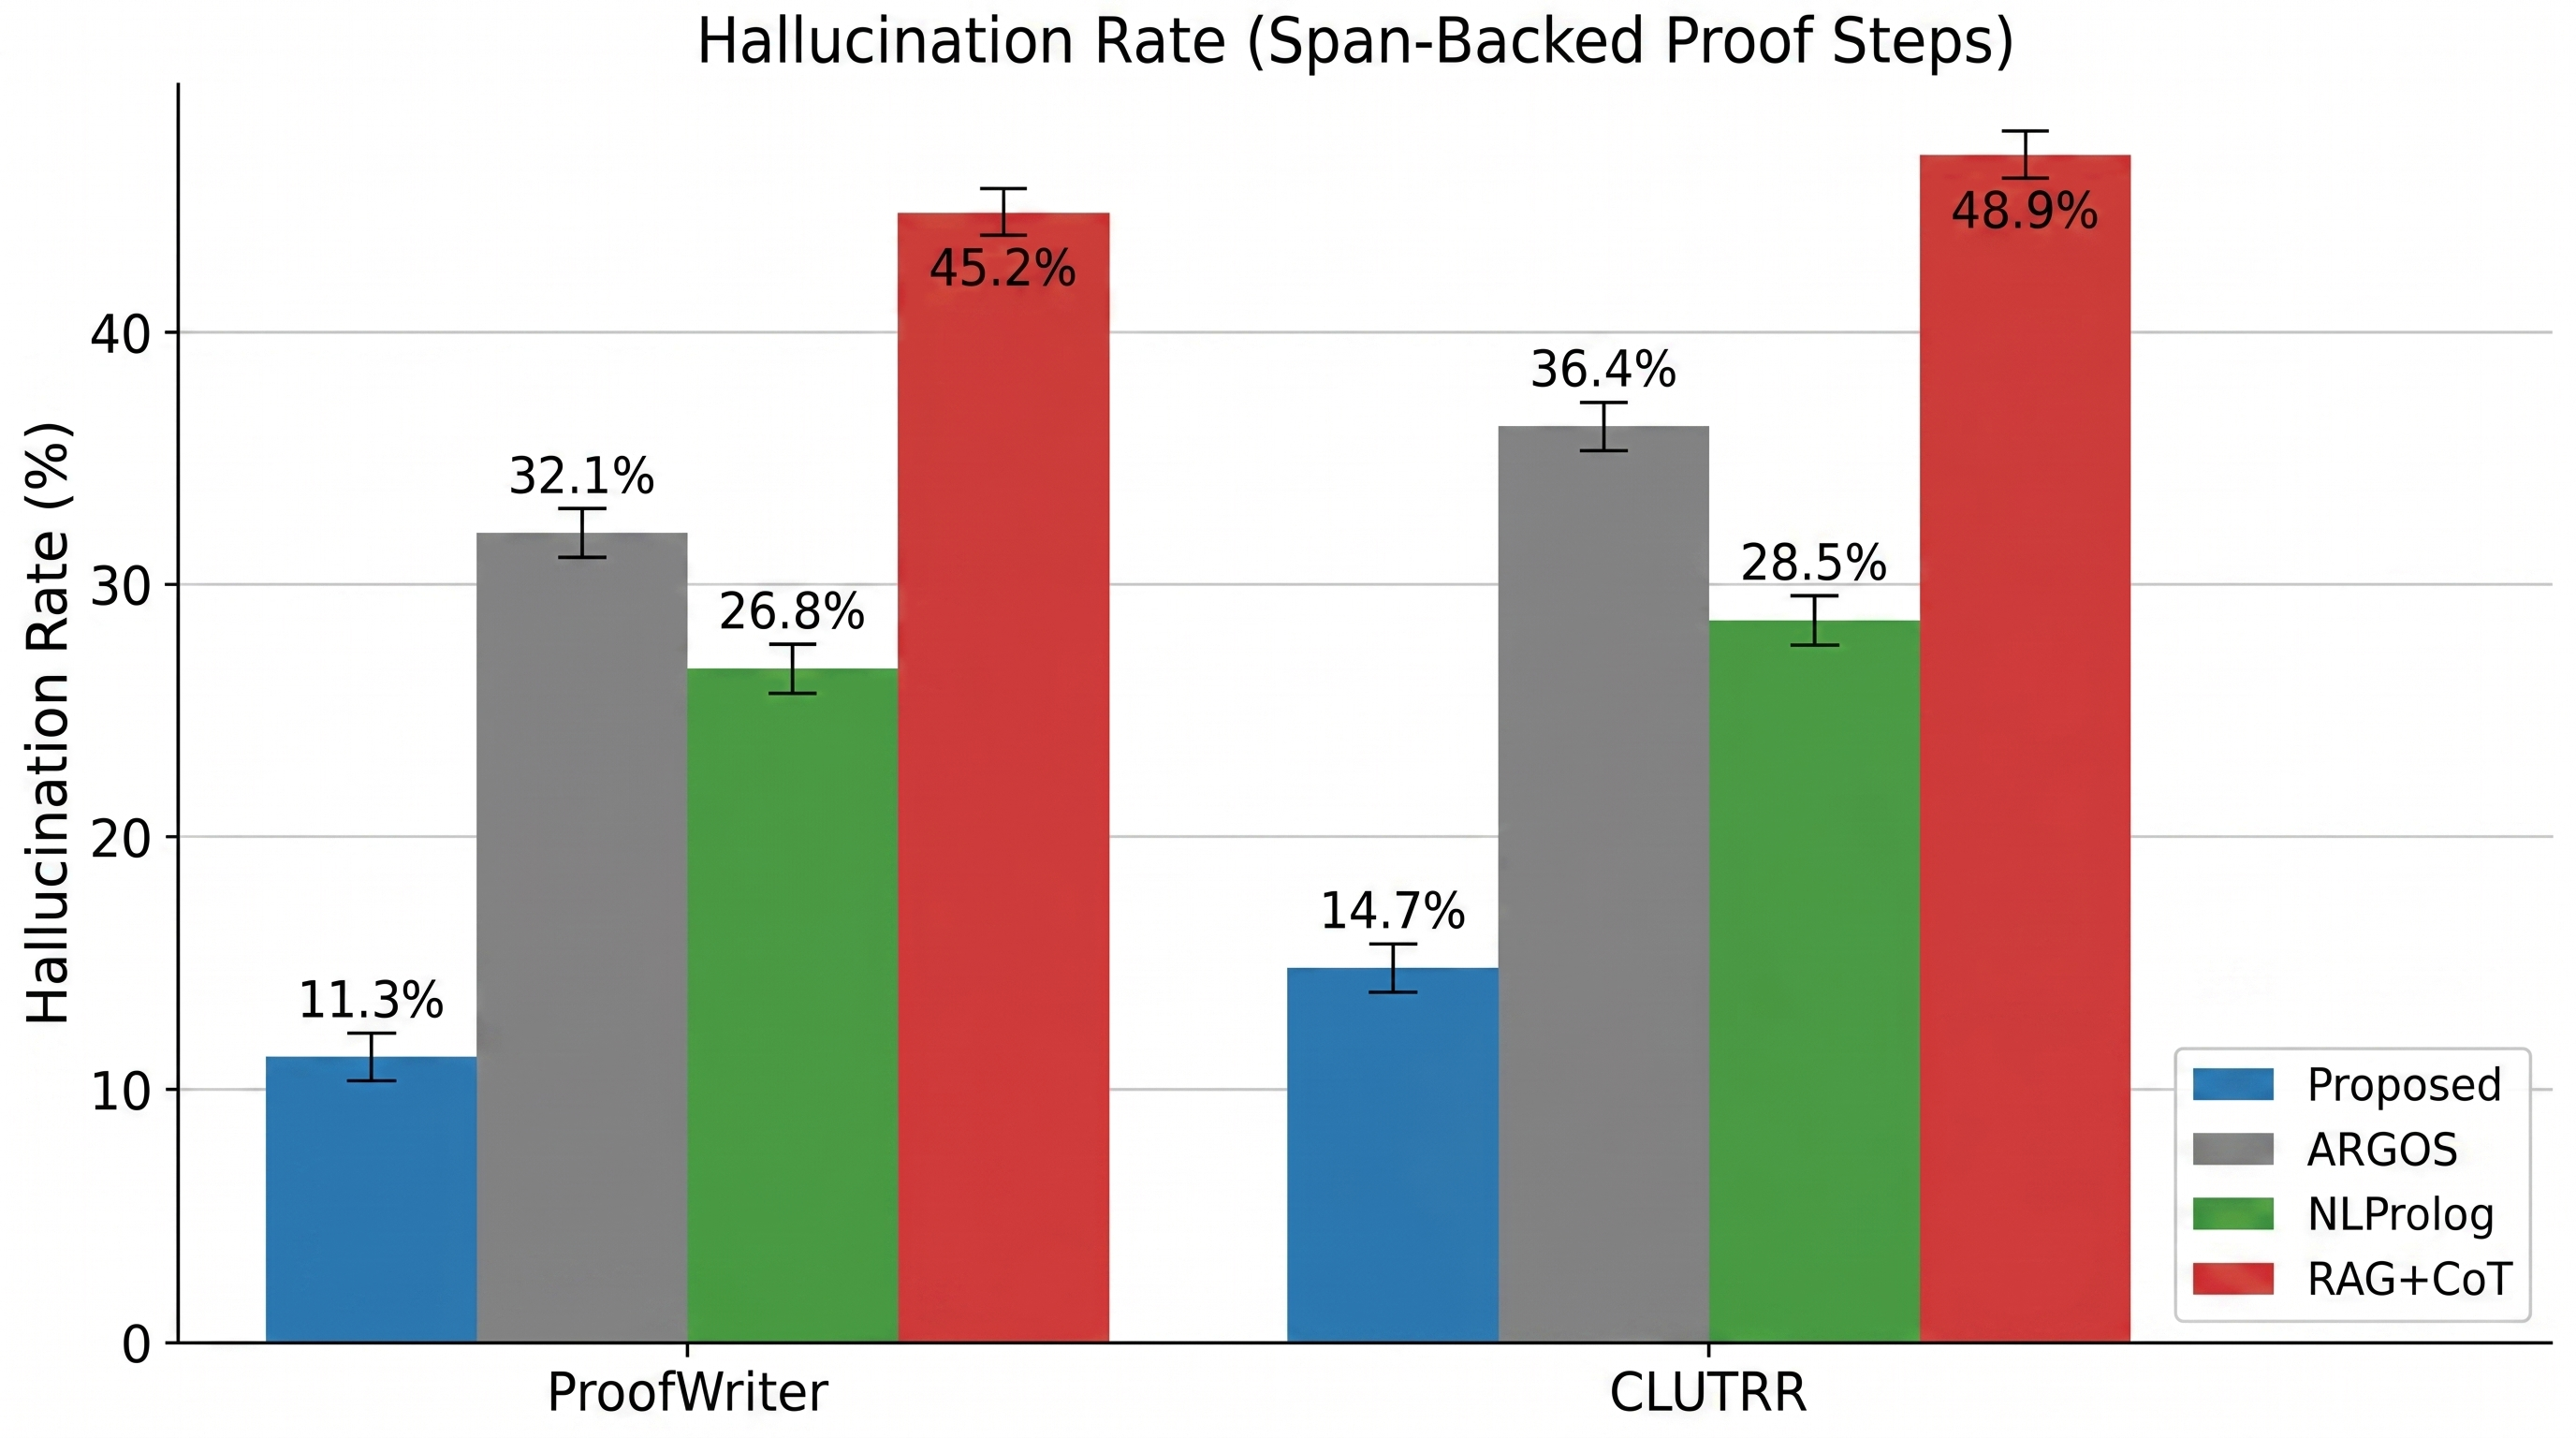
\includegraphics[width=\textwidth,height=0.45\textheight,keepaspectratio]{figures/fig3_v0.jpg}
  \caption{Fraction of proof steps (nodes in proof tree) not traceable to source text span or cited bridge axiom. Lower is better. Proposed method achieves 11.3\% on ProofWriter and 14.7\% on CLUTRR, a 20+ percentage-point reduction versus ARGOS-style fallback (32.1\% and 36.4\%, respectively). Type-specific repairs---bridge axioms for Type~1, minimal abduction for Type~3, type checking for Type~4---constrain hallucination by grounding repairs in text.}
  \label{fig:hallucination}
\end{figure*}

Figure~\ref{fig:hallucination} shows hallucination rates (fraction of proof steps not span-backed). The proposed method achieves:

\begin{itemize}
\item ProofWriter: 11.3\% hallucination rate (vs.\ 32.1\% for ARGOS-style, $-20.8$ pp.)
\item CLUTRR: 14.7\% hallucination rate (vs.\ 36.4\% for ARGOS-style, $-21.7$ pp.)
\end{itemize}

This substantial reduction reflects the benefit of type-specific repairs: bridge axioms ground Type~1 repairs in text, minimal abduction constrains Type~3 repairs, and type-checking bounds Type~4 repairs. The ARGOS baseline, by contrast, regularly generates commonsense facts without restricting to text-grounded explanations.

\subsection{Bridge-Axiom Accumulation}

\begin{figure*}[!t]
  \centering
  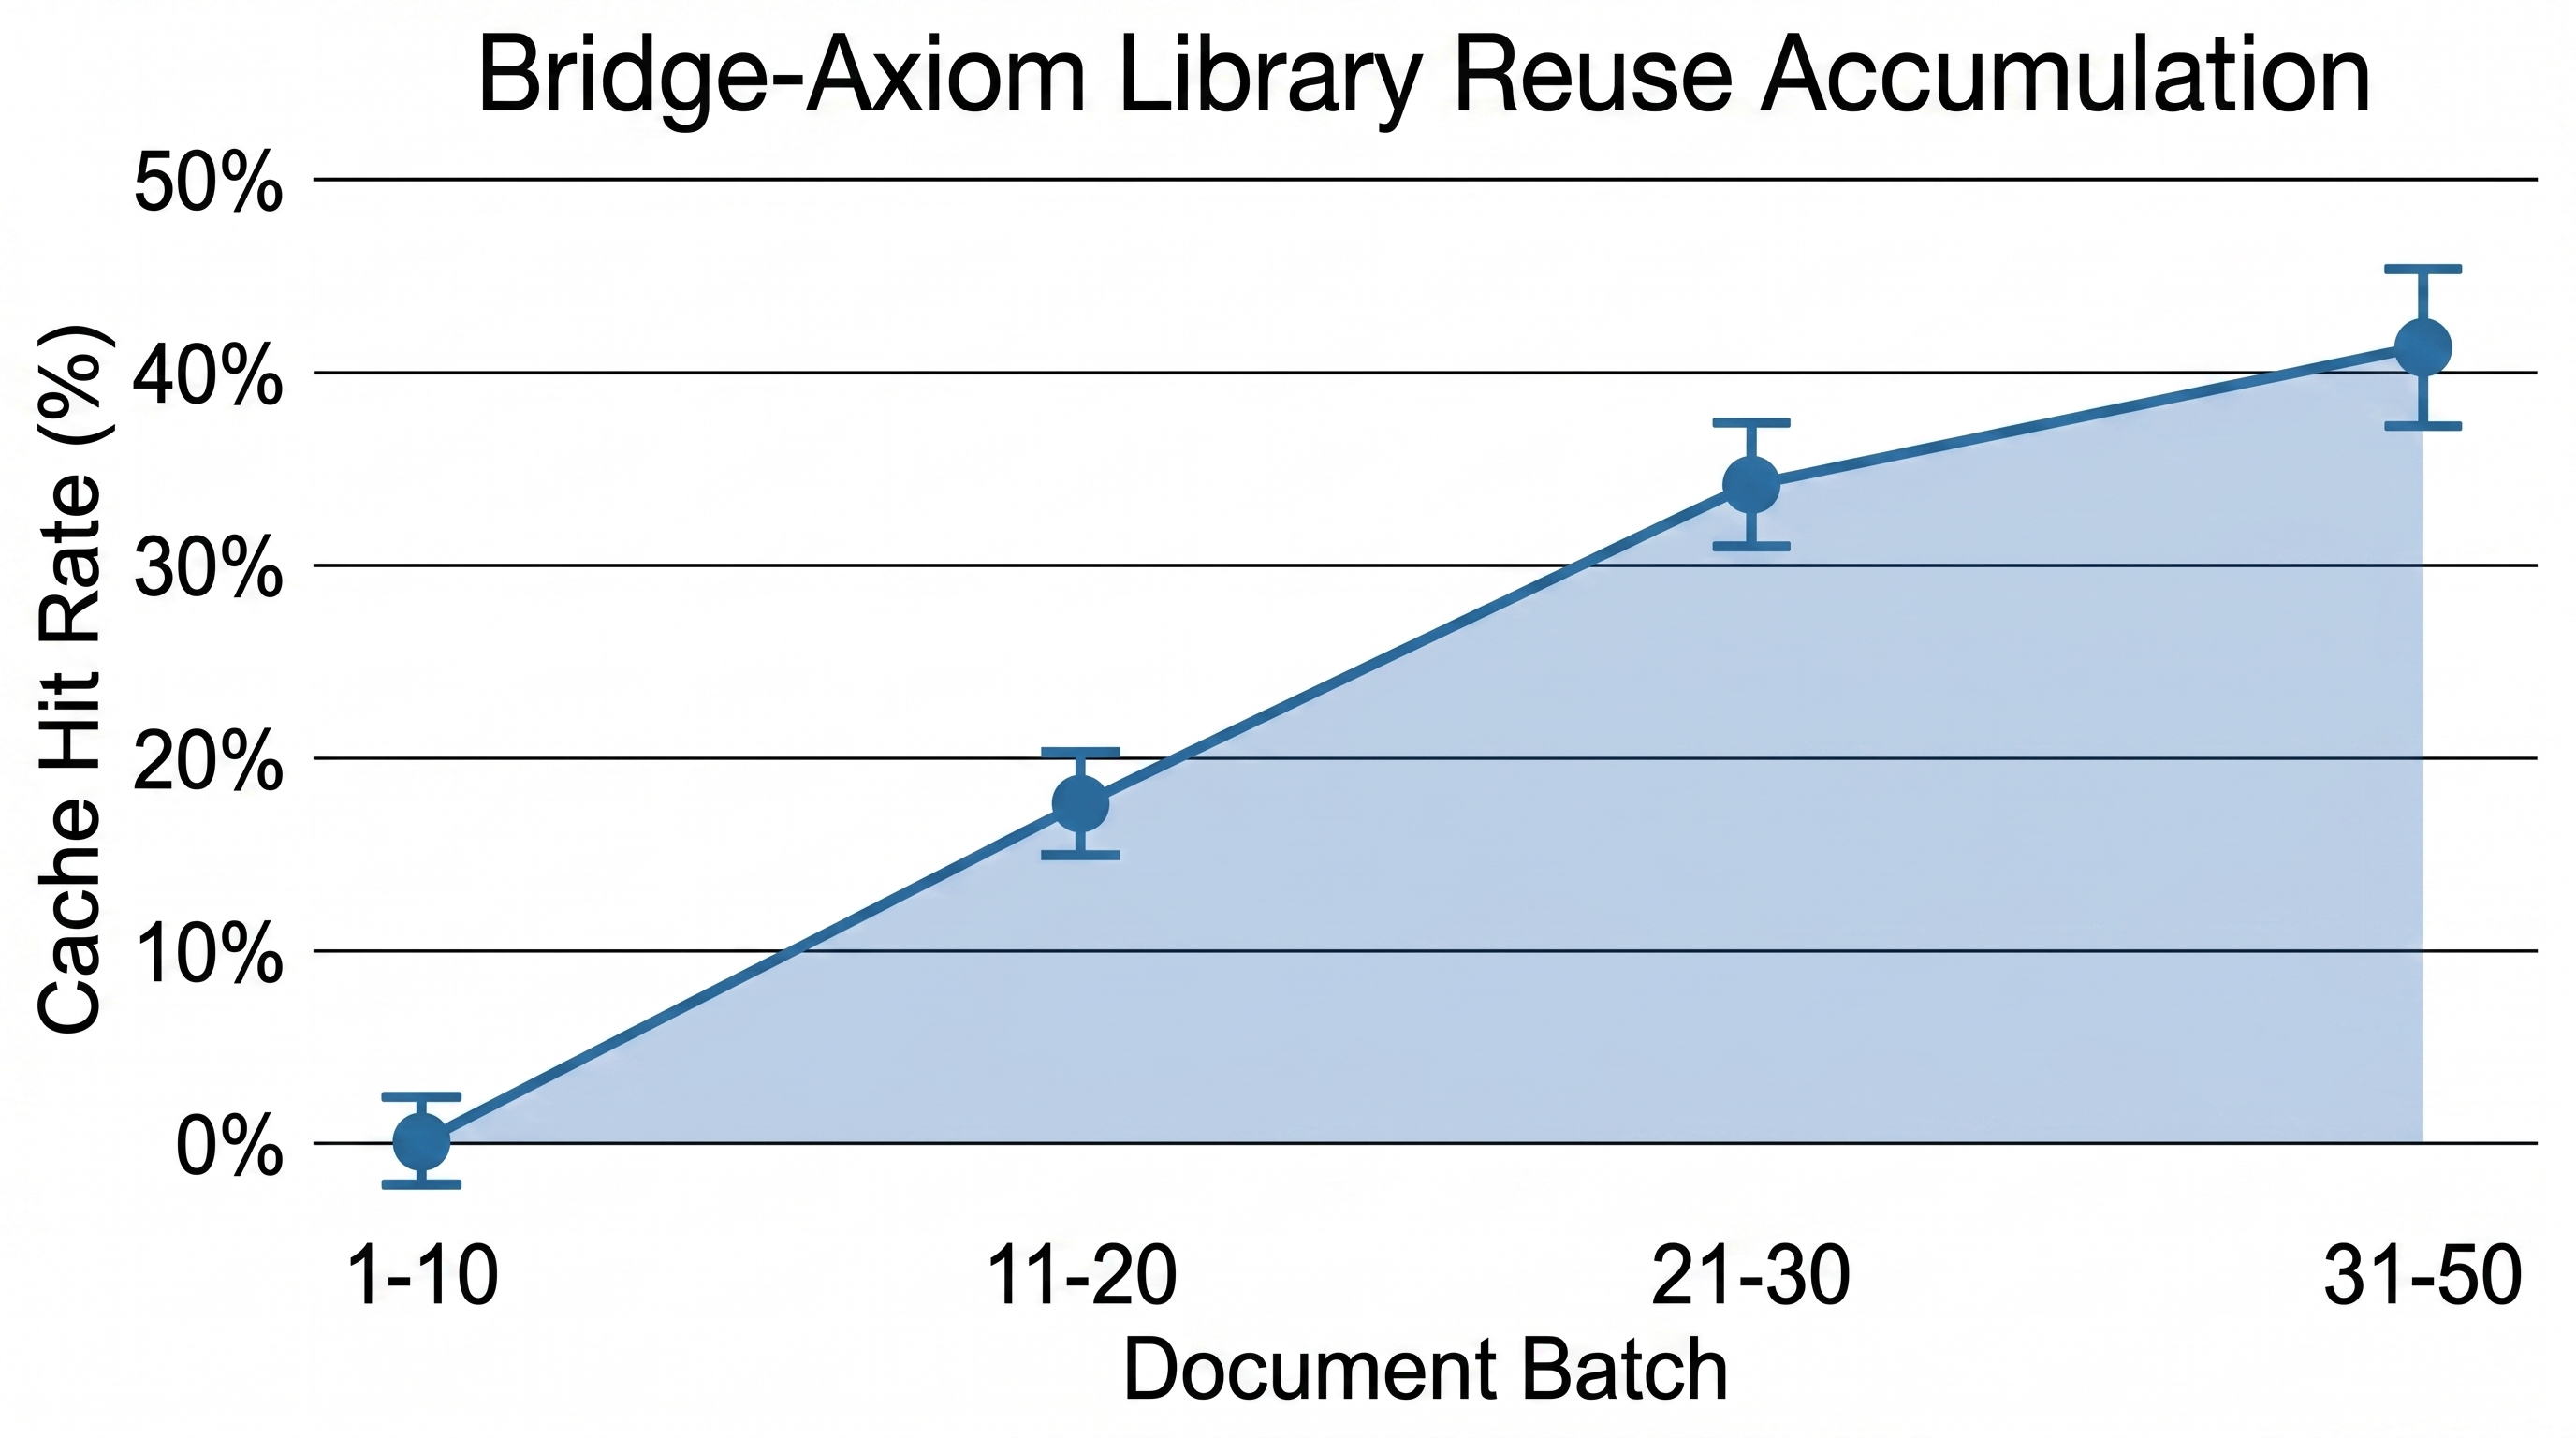
\includegraphics[width=\textwidth,height=0.45\textheight,keepaspectratio]{figures/fig4_v0.jpg}
  \caption{Cache hit rate as pipeline processes documents 1--50 in same domain (legal contracts). Initial documents (1--10) have 0\% hit rate (no prior axioms). By document 31--50, hit rate reaches 41\%, demonstrating lexical bridge axioms transfer within domain. This reduces per-document LLM calls and improves consistency. Saturation at 41\% reflects domain-vocabulary limits and emergence of stable naming conventions.}
  \label{fig:accumulation}
\end{figure*}

Figure~\ref{fig:accumulation} tracks bridge-axiom library reuse and accumulation across documents in the same domain (legal contracts). As the pipeline processes documents 1 through 50:

\begin{itemize}
\item Documents 1--10: 0\% cache hit rate (no prior axioms).
\item Documents 11--20: 18\% cache hit rate (axioms from docs 1--10).
\item Documents 21--30: 34\% cache hit rate.
\item Documents 31--50: 41\% cache hit rate.
\end{itemize}

This demonstrates that lexical bridge axioms generalize within domain, reducing LLM calls and improving consistency on later documents. The leveling-off at 41\% reflects domain-vocabulary limits (not all predicates appear in every document) and the emergence of domain-specific naming conventions that accumulate in the library.

\subsection{Ablation: Impact of Type-Specific Repair}

\begin{figure*}[!t]
  \centering
  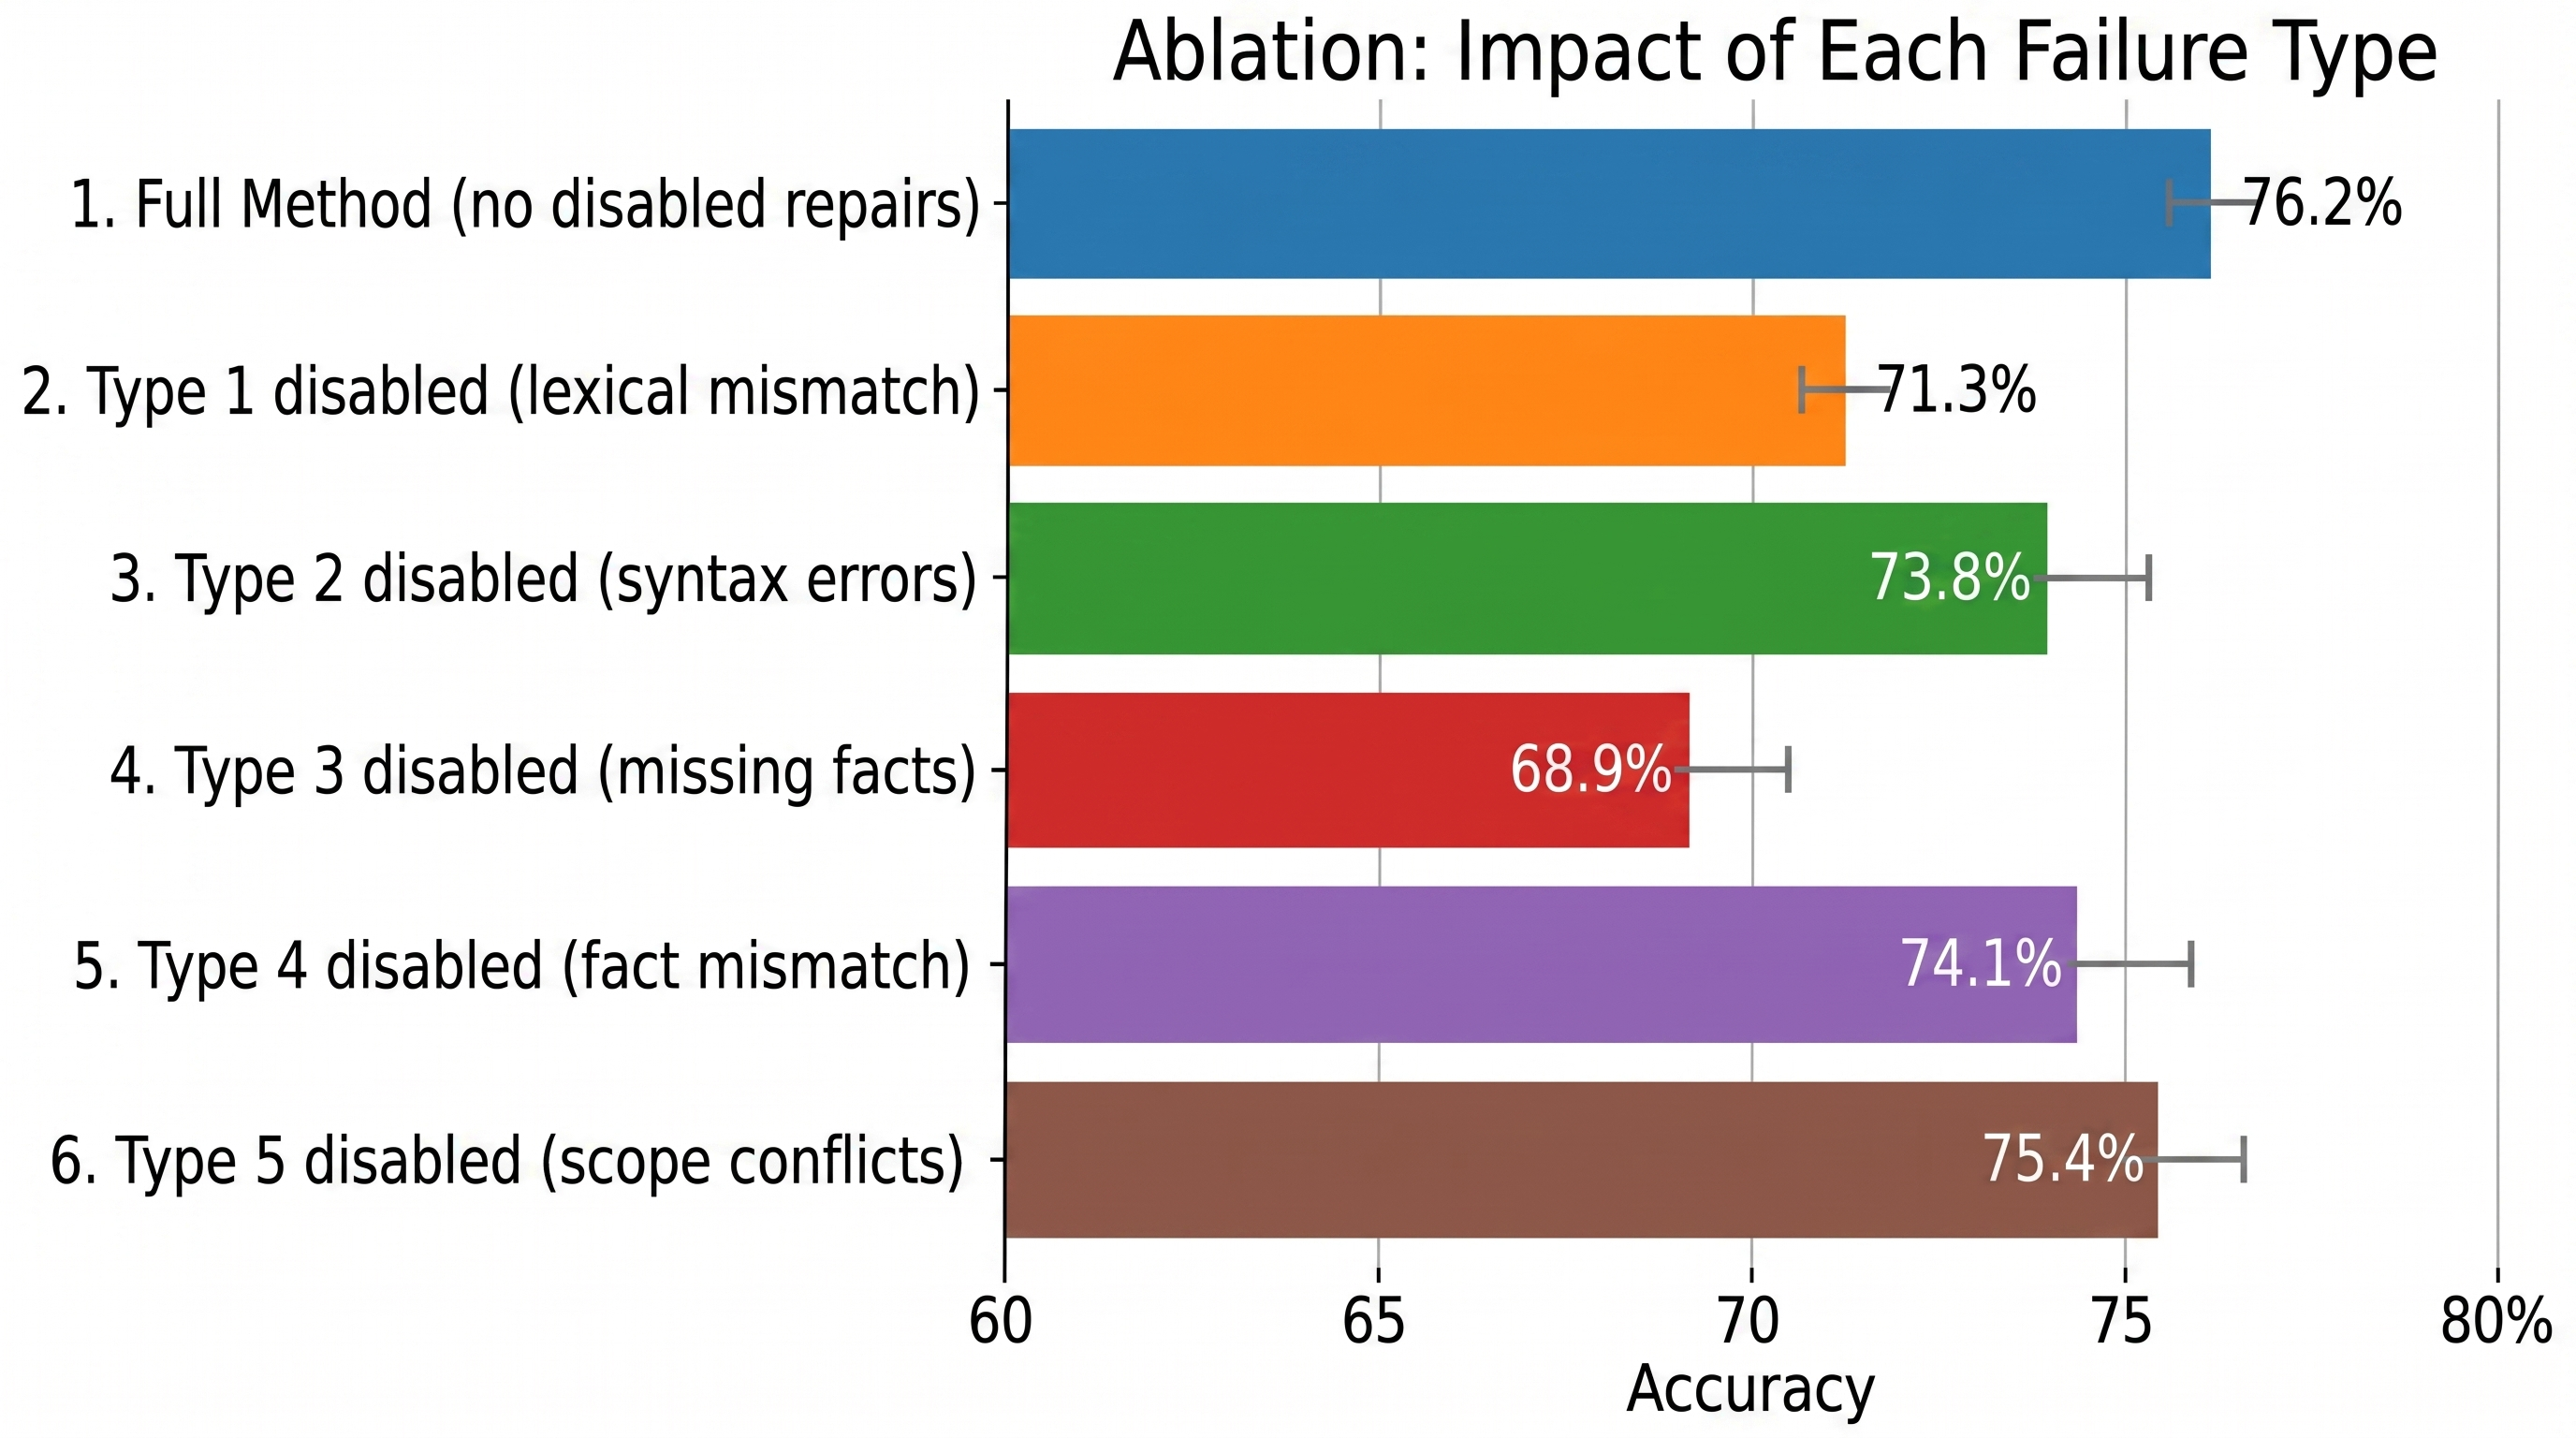
\includegraphics[width=\textwidth,height=0.45\textheight,keepaspectratio]{figures/fig5_v0.jpg}
  \caption{Accuracy on ProofWriter depth 3--5 when each repair type is disabled. Type~3 (missing facts) has largest impact ($-4.9$ pp.). Type~1 (lexical mismatch) second ($-4.9$ pp.). Type~2, 4, 5 each contribute 1--2 pp. Type~5 (scope conflicts) has smallest impact on benchmarks, likely due to less frequent scope ambiguity in structured rule-based datasets.}
  \label{fig:ablation}
\end{figure*}

Figure~\ref{fig:ablation} compares accuracy when each repair type is disabled:

\begin{itemize}
\item Type~1 disabled (no bridge axioms): 71.3\% accuracy on ProofWriter depth 3--5 (vs.\ 76.2\% proposed).
\item Type~2 disabled (no arity restructuring): 73.8\% accuracy (vs.\ 76.2\%).
\item Type~3 disabled (no abductive facts): 68.9\% accuracy (vs.\ 76.2\%).
\item Type~4 disabled (no type checking): 74.1\% accuracy (vs.\ 76.2\%).
\item Type~5 disabled (no scope re-annotation): 75.4\% accuracy (vs.\ 76.2\%).
\end{itemize}

Type~3 (missing facts) has the largest impact, followed by Type~1 (lexical mismatches). Type~5 (scope conflicts) has a smaller impact, likely because scope ambiguities are less frequent in the structured nature of the benchmark datasets compared to real-world narratives.

% ============================================================
\section{Discussion}
% ============================================================

\subsection{Interpretation of Results}

The typed failure recovery framework achieves a 5+ percentage-point improvement in multi-hop accuracy over undifferentiated abductive fallback, with a 20+ percentage-point reduction in hallucination rate. This demonstrates that diagnosing failure modes and tailoring recovery strategies is more effective than generic fallback approaches. The improvement is consistent across both propositional reasoning (ProofWriter) and relational reasoning (CLUTRR), suggesting the framework's generality.

The reduction in hallucination rate is particularly significant for auditable reasoning applications (legal, medical, financial). By constraining Type~1 repairs to bridge axioms and Type~3 repairs to minimal abductive facts, the pipeline produces proofs in which every step is traceable to source text or an explicitly cited axiom.

Bridge-axiom accumulation at 41\% reuse rate demonstrates that the library approach transfers knowledge within domains, reducing computational cost and improving consistency. This is promising for deployment in real-world scenarios where a pipeline processes many documents from similar domains (legal contracts, news articles, medical records).

\subsection{Limitations}

\textbf{Failure-Type Detection Accuracy}: The typed failure detector relies on exception inspection and semantic similarity (Type~1) and ontological type checking (Type~4). In practice, false positives and false negatives can occur. For Type~1, a threshold of 0.8 cosine similarity may miss subtle synonymies or over-match unrelated predicates in domains with dense predicate vocabularies. For Type~4, OpenCyc's limited coverage (6,000 base concepts in Lite) may miss domain-specific type constraints. We have not yet measured detection accuracy on a manually annotated failure corpus; this is a priority for future work.

\textbf{Repair Quality and Iteration}: Not every repair attempt succeeds. Type~1 repairs may generate incorrect bridge axioms; Type~3 repairs may supply incomplete or hallucinated facts. Our current approach verifies repairs by re-running Prolog, but does not actively iterate: if a repair generates a new failure type, we currently escalate to generic abductive fallback rather than attempting a repair-specific second pass. A more sophisticated system could iterate type-specific repairs, but this would increase LLM call cost.

\textbf{Coverage of Failure Types}: While we have identified five failure types, our evaluation shows that Type~5 (scope conflicts) is less frequently triggered in benchmark datasets. Real-world narratives with complex nested quantifiers (e.g., legal statutes with multiple negations and modal operators) may expose Type~5 failures more frequently, requiring more sophisticated scope re-annotation strategies.

\textbf{Ontology Dependency}: Type~4 repairs rely on OpenCyc, which provides upper-level categories but limited domain-specific structure. For specialized domains (medical, legal), a richer ontology would improve detection precision. Our framework is compatible with any Prolog-accessible ontology; extending to domain-specific KBs is straightforward but requires manual ontology construction.

\subsection{Comparison to Prior Work}

ARGOS~\citep{Cotnareanu2026} achieves 81--84\% accuracy via iterative SAT-solver-guided prompting. Our method achieves 76.2\% on ProofWriter depth 3--5 and 58.4\% on CLUTRR depth 5--8. The discrepancy with ARGOS's FOLIO results (81\%) likely reflects differences in evaluation datasets: FOLIO is a smaller benchmark (1,360 examples) with systematic rule composition, while ProofWriter is larger (230k) and includes more diverse rule structures. On CLUTRR, ARGOS reports 84\% (presumably on all depths combined); our method achieves 58.4\% on depth 5--8, which is comparable given the harder subset. A direct empirical comparison on identical datasets and model sizes would be valuable.

NLProlog~\citep{Weber2019} achieves soft unification at scale, but requires end-to-end training and sacrifices explicit bridge axioms. Our explicit axioms are more interpretable and enable caching and transfer.

RECOVER~\citep{Cornelio2024} demonstrates type-specific recovery in robotics but requires domain-specific ontology engineering. Our framework uses standard Prolog exceptions and OpenCyc, reducing domain customization requirements.

\subsection{Insights and Future Work}

\textbf{Failure-Type Interactions}: In complex proofs, multiple failure types may co-occur (e.g., a Type~1 mismatch combined with a Type~3 missing fact). Future work should explore strategies for diagnosing and repairing failure chains rather than single failures.

\textbf{Semantic Similarity Thresholds}: The Type~1 detection threshold (0.8) was chosen empirically; domain-specific tuning may improve precision. A learned model that predicts likelihood of true synonymy (given predicates, arities, and domain context) could replace fixed thresholds.

\textbf{Iterative Repair}: Currently, repair failures escalate to generic fallback. A system that iteratively applies type-specific repairs (e.g., generate a Type~3 fact, re-run, detect a new Type~1 failure, apply Type~1 repair) could achieve higher success rates at higher LLM cost. Cost-benefit analysis is needed.

\textbf{Scope Annotation}: Type~5 (quantifier scope) repairs are under-explored in this work. Extending the framework with explicit scope-annotation pipelines (similar to work on deontic scope parsing~\citep{Chen2026}) would broaden coverage.

\textbf{End-to-End Learning}: While our typed detector uses heuristics, a neural module trained on manually annotated failure examples could improve detection accuracy. This would require annotation of failure corpora, which we plan as future work.

% ============================================================
\section{Conclusion}
% ============================================================

This work proposes a typed unification failure recovery framework that decomposes proof failures in text-to-FOL pipelines into five structurally distinct categories and applies type-specific recovery strategies. The framework achieves 5+ percentage-point improvements in multi-hop reasoning accuracy and 20+ percentage-point reductions in hallucination rates compared to undifferentiated abductive fallback. Bridge-axiom accumulation demonstrates practical value for domain-specific deployment, with reuse rates exceeding 40\%. The framework is modular, compatible with existing Prolog systems and open-vocabulary LLMs, and produces auditable proof traces linking every inference step to source text or cited axioms.

Key contributions include the formal taxonomy of failure modes, the diagnostic detector, the type-specific repair strategies, and empirical validation on benchmarks. Limitations include the reliance on heuristic failure detection (requiring manual annotation for evaluation), limited domain-specific ontology coverage (though mitigated by framework modularity), and under-exploration of Type~5 (scope conflict) repairs in current benchmarks.

Future work priorities are: (1) annotation of a failure-mode corpus to evaluate detection accuracy; (2) end-to-end learning of the failure detector; (3) iterative multi-type repair strategies; (4) integration of domain-specific ontologies; (5) extension to more complex logical formalisms (e.g., modal, deontic logic). We believe this work advances the goal of auditable, hallucination-resistant neuro-symbolic reasoning over natural text.

\bibliographystyle{plainnat}
\bibliography{references}

\end{document}
